\documentclass[11pt,]{article}
\usepackage[left=1in,top=1in,right=1in,bottom=1in]{geometry}
\newcommand*{\authorfont}{\fontfamily{phv}\selectfont}

\usepackage[]{mathpazo}


  \usepackage[T1]{fontenc}
  \usepackage[utf8]{inputenc}

\usepackage{abstract}
\renewcommand{\abstractname}{}    % clear the title
\renewcommand{\absnamepos}{empty} % originally center

\renewenvironment{abstract}
 {{%
    \setlength{\leftmargin}{0mm}
    \setlength{\rightmargin}{\leftmargin}%
  }%
  \relax}
 {\endlist}

\makeatletter
\def\@maketitle{%
  \newpage
%  \null
%  \vskip 2em%
%  \begin{center}%
  \let \footnote \thanks
    {\fontsize{18}{20}\selectfont\raggedright  \setlength{\parindent}{0pt} \@title \par}%
}
%\fi
\makeatother




\setcounter{secnumdepth}{0}


\usepackage{graphicx,grffile}
\makeatletter
\def\maxwidth{\ifdim\Gin@nat@width>\linewidth\linewidth\else\Gin@nat@width\fi}
\def\maxheight{\ifdim\Gin@nat@height>\textheight\textheight\else\Gin@nat@height\fi}
\makeatother
% Scale images if necessary, so that they will not overflow the page
% margins by default, and it is still possible to overwrite the defaults
% using explicit options in \includegraphics[width, height, ...]{}
\setkeys{Gin}{width=\maxwidth,height=\maxheight,keepaspectratio}

\title{Lab 2: Algal bioassay: assessing nutrient limitation \thanks{\textbf{Current version}: February , 2019}  }



\author{\Large BIO 3103, Baylor University\vspace{0.05in} \newline\normalsize\emph{}  }


\date{}

\usepackage{titlesec}

\titleformat*{\section}{\Large\bfseries}
\titleformat*{\subsection}{\normalsize\itshape}
\titleformat*{\subsubsection}{\normalsize\itshape}
\titleformat*{\paragraph}{\normalsize\itshape}
\titleformat*{\subparagraph}{\normalsize\itshape}





\newtheorem{hypothesis}{Hypothesis}
\usepackage{setspace}

\makeatletter
\@ifpackageloaded{hyperref}{}{%
\ifxetex
  \PassOptionsToPackage{hyphens}{url}\usepackage[setpagesize=false, % page size defined by xetex
              unicode=false, % unicode breaks when used with xetex
              xetex]{hyperref}
\else
  \PassOptionsToPackage{hyphens}{url}\usepackage[unicode=true]{hyperref}
\fi
}

\@ifpackageloaded{color}{
    \PassOptionsToPackage{usenames,dvipsnames}{color}
}{%
    \usepackage[usenames,dvipsnames]{color}
}
\makeatother
\hypersetup{breaklinks=true,
            bookmarks=true,
            pdfauthor={BIO 3103, Baylor University ()},
             pdfkeywords = {},  
            pdftitle={Lab 2: Algal bioassay: assessing nutrient limitation},
            colorlinks=true,
            citecolor=blue,
            urlcolor=blue,
            linkcolor=magenta,
            pdfborder={0 0 0}}
\urlstyle{same}  % don't use monospace font for urls

% set default figure placement to htbp
\makeatletter
\def\fps@figure{htbp}
\setlength{\intextsep}{25pt}  % sets space after text/before float figure
\makeatother

\usepackage{multicol}
\usepackage{textcomp}


% add tightlist ----------
\providecommand{\tightlist}{%
\setlength{\itemsep}{0pt}\setlength{\parskip}{0pt}}

\begin{document}
	
% \pagenumbering{arabic}% resets `page` counter to 1 
%


% \maketitle

{% \usefont{T1}{pnc}{m}{n}
\setlength{\parindent}{0pt}
\thispagestyle{plain}
{\fontsize{18}{20}\selectfont\raggedright 
\maketitle  % title \par  

}

{
   \vskip 13.5pt\relax \normalsize\fontsize{11}{12} 
\textbf{\authorfont BIO 3103, Baylor University} \hskip 15pt \emph{\small }   

}

}




\noindent  \section{Background information}\label{background-information}

All organisms need certain resources in order to survive. For primary
producers (organisms that fix inorganic carbon using light energy), the
nutrients nitrogen (N) and phosphorus (P) are vital for growth and
reproduction. N exists in large supply in the atmosphere
(\textasciitilde{}78\%), but only a few specialized N-fixing organisms
can access this inorganic N pool. The primary source of P in the
environment is decomposing organic-P, and the weathering of inorganic P
from P-rich rocks. One or both of these nutrients can limit growth if
the availability of N or P does not meet demand.

Aquatic algae are remarkably consistent in their elemental requirements.
For every molecule of P, algae generally require 16 molecules of N, and
106 molecules of carbon (C). The ratio of C:N:P in biomass is called the
Redfield ratio, and though there is some natural variation, most aquatic
algae generally display the ratio 106:16:1.

\begin{figure}
\centering
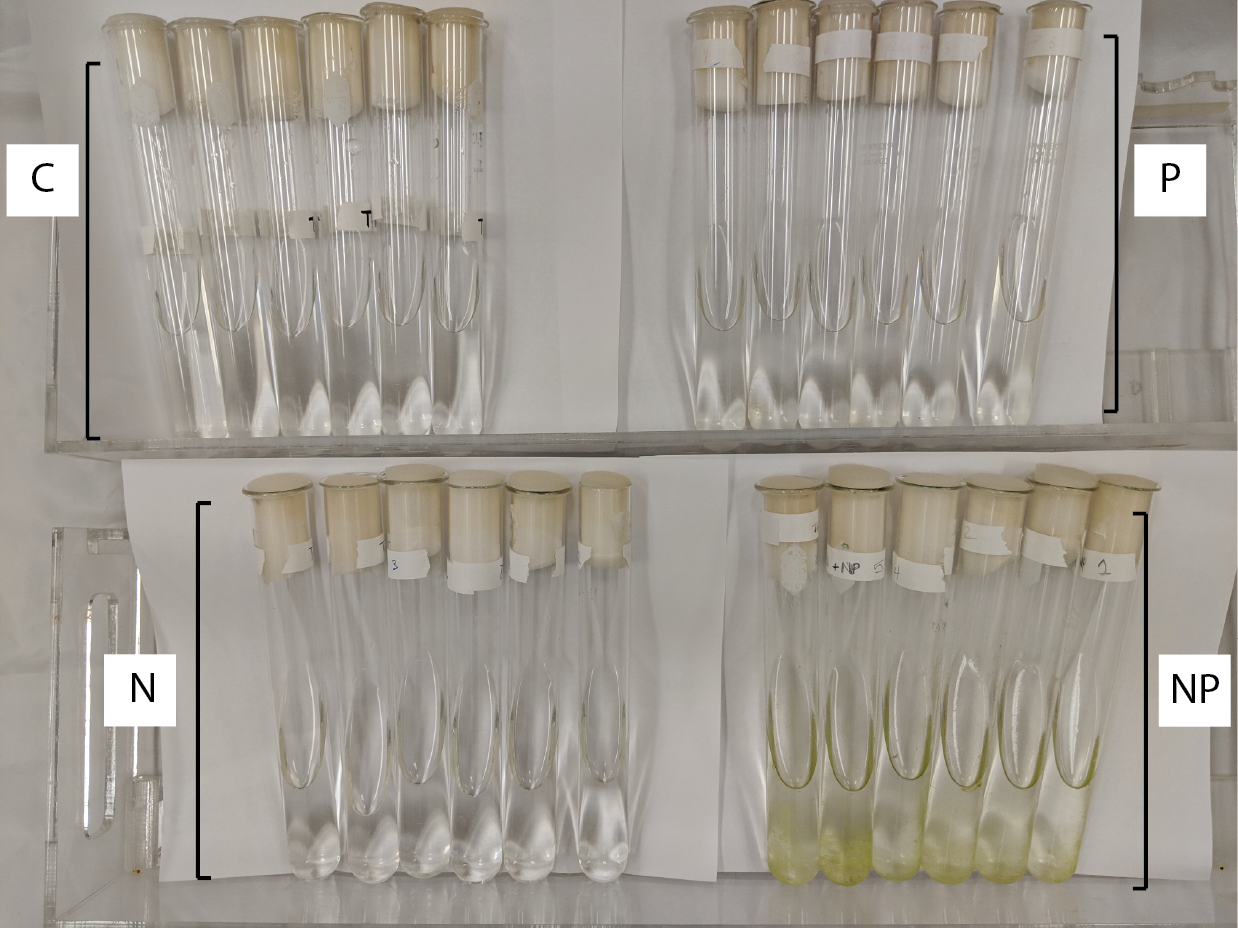
\includegraphics{../_chapter_materials/bioassay_picture.png}
\caption{Algal growth in borosilicate glass culture tubes 7 days after
start of incubations. C = control, N = nitrogen, P = phosphorus, NP =
nitrogen and phosphorus.}
\end{figure}

\section{Objectives}\label{objectives}

For this experiment you will ammend lake water with the macronutrients
nitrogen and phosphorus. By assessing how the algae community responds
to these treatments, you will be able to tell which (if any) nutrient is
limiting growth. \bigskip

\pagebreak

\subsection{Materials}\label{materials}

\begin{multicols}{2}
\begin{itemize}{}
  \item Borosilicate glass culture tubes
  \item Lake water sample (collect at least 30 mL per replicate)
  \item 0.01 M phosphorus solution \\(NaH\textsubscript{2}PO\textsubscript{4} \textbullet  H\textsubscript{2}O)
  \item 0.16 M nitrogen solution \\ (NaNO\textsubscript{3})
  \item Micropipette and disposable tips
  \item Light source (> 400 \textmu E m\textsuperscript{-2}s\textsuperscript{-1})
  \item Fluorometer
\end{itemize}
\end{multicols}

\subsection{Methods}\label{methods}

\begin{enumerate}
\def\labelenumi{\arabic{enumi}.}
\tightlist
\item
  Organize and label 6 culture tubes per nutrient treatment. There
  should be a nitrogen treatment, a phosphorus treatment, a nitrogen and
  phosphorus treatment, as well as a control (no nutrients should be
  added to the control).
\item
  Fill culture tubes with 30 mL of lake water.
\item
  Add 100 \(\mu\)L of nutrient solution according to treatment.
\item
  Mix combined solution in culture tubes by gently swirling. You may
  also use a vortex-mixer.
\item
  Fit a foam stopper in the top of each tube. This reduces the chance
  that organisms fall into the tubes during the incubation.
\item
  Take initial readings with the fluorometer.
\item
  Incubate for 1 week. Either take readings each day, or take final
  measurements on day 7.
\end{enumerate}

\subsection{Hypotheses}\label{hypotheses}

We will use this data to test hypotheses addressing the following
question:

\begin{itemize}
\tightlist
\item
  Is the algae community in our lake sample limited by nitrogen or
  phosphorus?

  \begin{itemize}
  \tightlist
  \item
    And if so, which one?
  \item
    Please form testable null hypotheses to address this question.
  \end{itemize}
\item
  You will address this hypothesis by plotting the data in bar/column
  graph form, then running an analysis of variance and Tukey post-hoc
  test.
\end{itemize}

\pagebreak

\section{Lab report specifics}\label{lab-report-specifics}

Below are some specific guidelines for this lab report, but you should
also utilize the general grading rubric in the Syllabus!

\begin{itemize}
\item
  \textbf{Participation} (1 pts)
\item
  \textbf{Introduction} (2 pts)

  \begin{itemize}
  \tightlist
  \item
    What factors can limit primary producers?
  \item
    Nutrients/redfield ratio?
  \item
    What is one method we can use to assess nutrient limitation (algal
    bioassay)?
  \item
    Objectives/hypothesis statement
  \end{itemize}
\item
  \textbf{Methods} (2 pts)

  \begin{itemize}
  \tightlist
  \item
    Explanation of data collection and analysis
  \end{itemize}
\item
  \textbf{Results} (5 pts)

  \begin{itemize}
  \tightlist
  \item
    Text section (overview of results, summary statistics, etc.)
  \item
    Bar-plot of fluorescence
  \item
    Statistics (anova, tukey post-hoc test)
  \end{itemize}
\item
  \textbf{Discussion} (2 pts)

  \begin{itemize}
  \tightlist
  \item
    Clearly address your null hypotheses
  \item
    What are some plausible explanations for differences (or lack
    thereof) between treatments?
  \item
    Relate this back to nutrients in the water column
  \item
    How might humans be influencing nutrient concentrations?
  \end{itemize}
\end{itemize}




\newpage
\singlespacing 
\end{document}
